\documentclass[border=10mm]{standalone}
% \usepackage[a4paper,top=2cm,bottom=2cm,left=2cm,right=2cm]{geometry}
\usepackage[margin=1in]{geometry}
\usepackage{graphicx}
\usepackage{bm}
\usepackage{pgfplots}
\usepackage{tikz}
\usetikzlibrary{calc}
\def\MarkRightAngle[size=#1](#2,#3,#4){
  \draw[] ($(#3)!#1!(#2)$) -- ($($(#3)!#1!(#2)$)!#1!90:(#2)$) -- ($(#3)!#1!(#4)$)
}

\usetikzlibrary{patterns}
\usetikzlibrary{angles,quotes}
\usepackage{parskip}
\usetikzlibrary{intersections, pgfplots.fillbetween}
\usepackage{amsmath}
\usepackage{multicol}
\usepackage{enumitem}
\usepackage{multirow}


\begin{document}


\tikzset{every picture/.style={line width=0.75pt}} %line width

\begin{tikzpicture}[x=0.75pt,y=0.75pt,yscale=-1,xscale=1]

%Rectangles
\draw   (126.67,129.67) -- (212.33,129.67) -- (212.33,182.67) -- (126.67,182.67) -- cycle ;
\draw   (386.67,129.33) -- (459.67,129.33) -- (459.67,182.33) -- (386.67,182.33) -- cycle ;

%Straight lines
\draw    (212.33,135.67) -- (387,135.67) ;
\draw    (212.33,163.67) -- (387,163.67) ;
\draw    (212.33,143.67) -- (243,143.67) ;
\draw    (212.33,149.67) -- (243,149.67) ;
\draw    (349.33,142.67) -- (387,142.67) ;
\draw    (349.33,149.67) -- (387,149.67) ;
\draw    (349.33,156.67) -- (387,156.67) ;
\draw    (459.67,136.33) -- (519.67,113.33) ;
\draw    (524.33,111.67) -- (559.33,97.67) ;
\draw    (459.67,141.33) -- (513.67,128) ;
\draw    (459.67,149.33) -- (513.67,138) ;
\draw    (459.33,176.33) -- (519.33,200.33) ;
\draw    (524.33,201.67) -- (559.33,216.67) ;
\draw    (90.33,136) -- (126.67,135.67) ;
\draw    (90.33,150) -- (126.67,149.67) ;
\draw    (90.33,177) -- (126.67,176.67) ;
\draw    (69,213.33) -- (37,155.33) ;
\draw    (157,269.33) -- (165.67,269.33) ;
\draw    (200.67,315.33) -- (222.33,315.33) ;
\draw    (577.67,316) -- (615,226) ;

%Ellipse Crosstalk
\draw   (359,150) .. controls (359,140.43) and (361.98,132.67) .. (365.67,132.67) .. controls (369.35,132.67) and (372.33,140.43) .. (372.33,150) .. controls (372.33,159.57) and (369.35,167.33) .. (365.67,167.33) .. controls (361.98,167.33) and (359,159.57) .. (359,150) -- cycle ;

%Half Ellipse dashed (Crosstalk)
\draw  [draw opacity=0][dash pattern={on 4.5pt off 4.5pt}] (474.32,182.65) .. controls (474.21,182.66) and (474.11,182.67) .. (474,182.67) .. controls (468.29,182.67) and (463.67,170.73) .. (463.67,156) .. controls (463.67,141.27) and (468.29,129.33) .. (474,129.33) .. controls (474.11,129.33) and (474.22,129.34) .. (474.33,129.35) -- (474,156) -- cycle ; \draw  [dash pattern={on 4.5pt off 4.5pt}] (474.32,182.65) .. controls (474.21,182.66) and (474.11,182.67) .. (474,182.67) .. controls (468.29,182.67) and (463.67,170.73) .. (463.67,156) .. controls (463.67,141.27) and (468.29,129.33) .. (474,129.33) .. controls (474.11,129.33) and (474.22,129.34) .. (474.33,129.35) ;  

%Half Ellipse (Crosstalk)
\draw  [draw opacity=0] (474.83,182.66) .. controls (474.94,182.67) and (475.04,182.67) .. (475.15,182.67) .. controls (480.22,182.67) and (484.33,170.73) .. (484.33,156.01) .. controls (484.33,141.28) and (480.22,129.34) .. (475.15,129.34) .. controls (475.04,129.34) and (474.93,129.34) .. (474.81,129.36) -- (475.15,156.01) -- cycle ; \draw   (474.83,182.66) .. controls (474.94,182.67) and (475.04,182.67) .. (475.15,182.67) .. controls (480.22,182.67) and (484.33,170.73) .. (484.33,156.01) .. controls (484.33,141.28) and (480.22,129.34) .. (475.15,129.34) .. controls (475.04,129.34) and (474.93,129.34) .. (474.81,129.36) ;  

%Arrow Lines
\draw[-stealth]    (168.83,129.17) -- (168.83,104.17) ;
\draw[-stealth]    (258.83,134.5) -- (258.83,113.5) ;
\draw[-stealth]    (311,102.33) -- (311,132.33) ;
\draw[-stealth]    (365.67,111.67) -- (365.67,129.67) ;
\draw[-stealth]    (423.17,129.17) -- (423.17,92.17) ;
\draw[-stealth]    (474.33,110.35) -- (474.33,126.35) ;
\draw[-stealth]    (508.83,117.83) -- (508.83,87.83) ;
\draw[-stealth]    (544.67,64.33) -- (544.67,100.33) ;
\draw[-stealth]    (568.17,90.5) -- (568.17,50.5) ;
\draw[-stealth]    (37,155.33) -- (51.67,155.33) ;
\draw[-stealth]    (165.67,269.33) -- (160.52,188.33) ;
\draw[-stealth]    (222.33,315.33) -- (186.48,188.22) ;
\draw[-stealth]    (247.67,223.33) -- (250.72,214.18) ;
\draw[-stealth]    (332.67,280) -- (299.04,215) ;
\draw[-stealth]    (351.67,237.33) -- (326.81,213.09) ;
\draw[-stealth]    (439.67,194.67) -- (432.93,186.63) ;
\draw[-stealth]    (490.33,303.33) -- (553.71,229.61) ;
\draw[stealth-]    (600.33,226) -- (615,226) ;

%Dotted lines
\draw  [dash pattern={on 0.84pt off 2.51pt}]  (232.33,152.33) -- (232.33,162.33) ;
\draw  [dash pattern={on 0.84pt off 2.51pt}]  (492,154) -- (492,164) ;
\draw  [dash pattern={on 0.84pt off 2.51pt}]  (567.33,127.33) -- (567.33,137.33) ;
\draw  [dash pattern={on 0.84pt off 2.51pt}]  (567.33,154.33) -- (567.33,164.33) ;
\draw  [dash pattern={on 0.84pt off 2.51pt}]  (567.33,181.33) -- (567.33,191.33) ;
\draw  [dash pattern={on 0.84pt off 2.51pt}]  (590.33,127.33) -- (590.33,137.33) ;
\draw  [dash pattern={on 0.84pt off 2.51pt}]  (590.33,154.33) -- (590.33,164.33) ;
\draw  [dash pattern={on 0.84pt off 2.51pt}]  (590.33,181.33) -- (590.33,191.33) ;
\draw  [dash pattern={on 0.84pt off 2.51pt}]  (107.33,158.67) -- (107.33,168.67) ;


%Human Icon
\draw (251.17,194) node  {
\includegraphics[width=18.25pt,height=20pt]{pic5.png}};
\draw (287.17,194) node  {
\includegraphics[width=18.25pt,height=20pt]{pic5.png}};
\draw (321.17,194) node  {
\includegraphics[width=18.25pt,height=20pt]{pic5.png}};
\draw (588.17,213) node  {
\includegraphics[width=18.25pt,height=20pt]{pic5.png}};
\draw (588.17,94) node  {
\includegraphics[width=18.25pt,height=20pt]{pic5.png}};
 

%Controller Icon
\draw (565.33,99.33) node [xscale=-1]{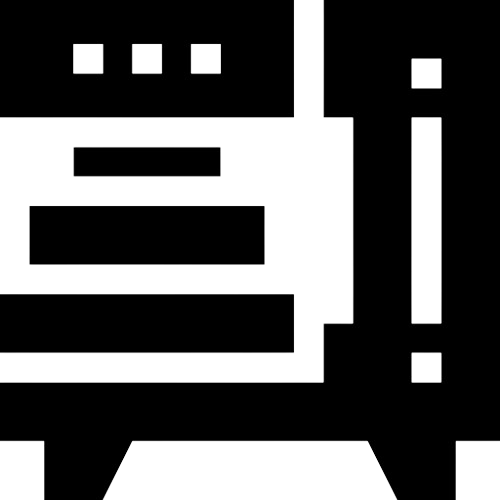
\includegraphics[width=7.5pt,height=12pt]{pic4.png}};
\draw (565.33,219.33) node [xscale=-1] {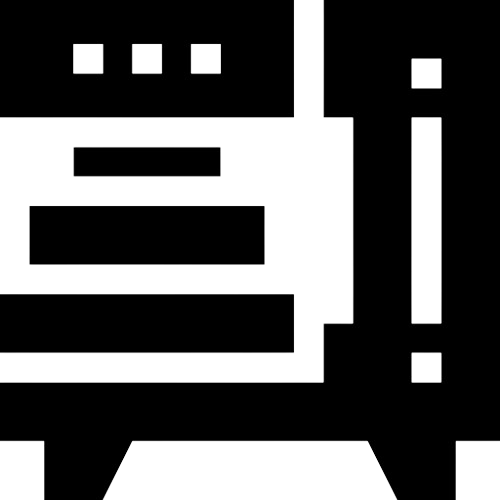
\includegraphics[width=7.5pt,height=12pt]{pic4.png}};


%Circles
\draw   (80.83,136) .. controls (80.83,133.38) and (82.96,131.25) .. (85.58,131.25) .. controls (88.21,131.25) and (90.33,133.38) .. (90.33,136) .. controls (90.33,138.62) and (88.21,140.75) .. (85.58,140.75) .. controls (82.96,140.75) and (80.83,138.62) .. (80.83,136) -- cycle ;
\draw   (80.83,150) .. controls (80.83,147.38) and (82.96,145.25) .. (85.58,145.25) .. controls (88.21,145.25) and (90.33,147.38) .. (90.33,150) .. controls (90.33,152.62) and (88.21,154.75) .. (85.58,154.75) .. controls (82.96,154.75) and (80.83,152.62) .. (80.83,150) -- cycle ;
\draw   (80.83,177) .. controls (80.83,174.38) and (82.96,172.25) .. (85.58,172.25) .. controls (88.21,172.25) and (90.33,174.38) .. (90.33,177) .. controls (90.33,179.62) and (88.21,181.75) .. (85.58,181.75) .. controls (82.96,181.75) and (80.83,179.62) .. (80.83,177) -- cycle ;
\draw   (76.08,136) .. controls (76.08,133.38) and (78.21,131.25) .. (80.83,131.25) .. controls (83.46,131.25) and (85.58,133.38) .. (85.58,136) .. controls (85.58,138.62) and (83.46,140.75) .. (80.83,140.75) .. controls (78.21,140.75) and (76.08,138.62) .. (76.08,136) -- cycle ;
\draw   (76.08,150) .. controls (76.08,147.38) and (78.21,145.25) .. (80.83,145.25) .. controls (83.46,145.25) and (85.58,147.38) .. (85.58,150) .. controls (85.58,152.62) and (83.46,154.75) .. (80.83,154.75) .. controls (78.21,154.75) and (76.08,152.62) .. (76.08,150) -- cycle ;
\draw   (76.08,177) .. controls (76.08,174.38) and (78.21,172.25) .. (80.83,172.25) .. controls (83.46,172.25) and (85.58,174.38) .. (85.58,177) .. controls (85.58,179.62) and (83.46,181.75) .. (80.83,181.75) .. controls (78.21,181.75) and (76.08,179.62) .. (76.08,177) -- cycle ;

% Curly brace
\draw   (68.33,126.67) .. controls (63.67,126.77) and (61.39,129.15) .. (61.49,133.82) -- (61.77,146.33) .. controls (61.92,152.99) and (59.67,156.37) .. (55,156.48) .. controls (59.67,156.37) and (62.07,159.65) .. (62.22,166.32)(62.16,163.32) -- (62.51,178.83) .. controls (62.61,183.49) and (64.99,185.77) .. (69.66,185.67) ;





%Text nodes

\draw (169.5,98.17) node [anchor=south] [inner sep=0.75pt]   [align=left] {\textbf{{\scriptsize RADIATION}}};

\draw (258.83,107.5) node [anchor=south] [inner sep=0.75pt]   [align=left] {\textbf{{\scriptsize RADIATION}}};

\draw (169.5,156.17) node  [font=\tiny] [align=left] {\textbf{PROCESSOR}};

\draw (423.17,155.83) node  [font=\tiny] [align=left] {\begin{minipage}[lt]{43.57pt}\setlength\topsep{0pt}
\begin{center}
\textbf{SWITCHING}\\\textbf{CENTER}
\end{center}

\end{minipage}};

\draw (297.67,138.67) node [anchor=north] [inner sep=0.75pt]  [font=\tiny] [align=left] {\begin{minipage}[lt]{64.46pt}\setlength\topsep{0pt}
\begin{center}
\textbf{COMMUNICATION}\\\textbf{LINES}
\end{center}

\end{minipage}};

\draw (311,99.33) node [anchor=south] [inner sep=0.75pt]  [font=\scriptsize] [align=left] {\textbf{TAPS}};

\draw (365.67,108.67) node [anchor=south] [inner sep=0.75pt]  [font=\scriptsize] [align=left] {\textbf{CROSSTALK}};

\draw (423.17,86.17) node [anchor=south] [inner sep=0.75pt]   [align=left] {\textbf{{\scriptsize RADIATION}}};

\draw (470.33,107.35) node [anchor=south] [inner sep=0.75pt]  [font=\scriptsize] [align=left] {\textbf{CROSSTALK}};

\draw (508.83,81.83) node [anchor=south] [inner sep=0.75pt]   [align=left] {\textbf{{\scriptsize RADIATION}}};

\draw (544.67,61.33) node [anchor=south] [inner sep=0.75pt]  [font=\scriptsize] [align=left] {\textbf{TAPS}};

\draw (568.17,44.5) node [anchor=south] [inner sep=0.75pt]   [align=left] {\textbf{{\scriptsize RADIATION}}};

\draw (71,213.33) node [anchor=west] [inner sep=0.75pt]   [align=left] {\begin{minipage}[lt]{19pt}\setlength\topsep{0pt}
\begin{center}
\textbf{{\scriptsize \underline{Files}}}
\end{center}

\end{minipage}};

\draw (247.67,221.33) node [anchor=north] [inner sep=0.75pt]   [align=left] {\begin{minipage}[lt]{42.53pt}\setlength\topsep{0pt}
\begin{center}
\textbf{{\scriptsize \underline{OPERATOR}}}
\end{center}

\end{minipage}};

\draw (208,243) node [anchor=north west][inner sep=0.75pt]  [font=\tiny] [align=left] {REPLACE SUPERVISOR\\REVEAL PROTECTIVE\\MEASURES};

\draw (49,220) node [anchor=north west][inner sep=0.75pt]  [font=\tiny] [align=left] {THEFT COPYING\\UNAUTHORIZED ACCESS};

\draw (439.67,190.67) node [anchor=north] [inner sep=0.75pt]   [align=left] {\begin{minipage}[lt]{44.77pt}\setlength\topsep{0pt}
\begin{center}
\textbf{\underline{{\scriptsize HARDWARE}}}
\end{center}

\end{minipage}};

\draw (407.67,213) node [anchor=north west][inner sep=0.75pt]  [font=\tiny] [align=left] {IMPROPER CONNECTIONS\\CROSS COUPLING};

\draw (140,267.33) node [anchor=east] [inner sep=0.75pt]   [align=left] {\begin{minipage}[lt]{44.77pt}\setlength\topsep{0pt}
\begin{center}
\textbf{\underline{{\scriptsize HARDWARE}}}
\end{center}

\end{minipage}};

\draw (62,279.67) node [anchor=north west][inner sep=0.75pt]  [font=\tiny] [align=left] {FAILURE OF PROTECTION\\ CIRCUITS CONTRIBUTE TO\\ SOFTWARE FAILURES};

\draw (188.67,313.33) node [anchor=east] [inner sep=0.75pt]   [align=left] {\begin{minipage}[lt]{43.18pt}\setlength\topsep{0pt}
\begin{center}
\textbf{\underline{{\scriptsize SOFTWARE}}}
\end{center}

\end{minipage}};

\draw (110,326) node [anchor=north west][inner sep=0.75pt]  [font=\tiny] [align=left] {FAILURE OF PROTECTION FEATURES\\ACCESS CONTROL BOUNDS CONTROL\\ETC.};

\draw (248.33,280.33) node [anchor=north west][inner sep=0.75pt]   [align=left] {\begin{minipage}[lt]{73.73pt}\setlength\topsep{0pt}
\begin{center}
\textbf{\underline{{\scriptsize MAINTENANCE MAN}}}
\end{center}

\end{minipage}};

\draw (248,301) node [anchor=north west][inner sep=0.75pt]  [font=\tiny] [align=left] {DISABLE HARDWARE DEVICES\\USE STAND-ALONE UTILITY PROGRAMS};

\draw (354.67,242.33) node [anchor=west] [inner sep=0.75pt]   [align=left] {\begin{minipage}[lt]{91.98pt}\setlength\topsep{0pt}
\begin{center}
\textbf{\underline{{\scriptsize SYSTEMS PROGRAMMER}}}
\end{center}

\end{minipage}};

\draw (354.67,253) node [anchor=north west][inner sep=0.75pt]  [font=\tiny] [align=left] {DISABLE PROTECTIVE FEATURES\\PROVIDE ``INS''\\REVEAL PROTECTIVE MEASURES};

\draw (488.33,303.33) node [anchor=east] [inner sep=0.75pt]   [align=left] {\begin{minipage}[lt]{32.48pt}\setlength\topsep{0pt}
\begin{center}
\textbf{\underline{{\scriptsize ACCESS}}}
\end{center}

\end{minipage}};

\draw (440,314) node [anchor=north west][inner sep=0.75pt]  [font=\tiny] [align=left] {ATTACHMENT OF \\RECORDERS BUGS};

\draw (547,235.33) node [anchor=north west][inner sep=0.75pt]  [font=\tiny] [align=left] {\begin{minipage}[lt]{31.34pt}\setlength\topsep{0pt}
\begin{center}
\textbf{REMOTE}\\\textbf{CONSOLES}
\end{center}

\end{minipage}};

\draw (575.67,316) node [anchor=east] [inner sep=0.75pt]   [align=left] {\begin{minipage}[lt]{22.57pt}\setlength\topsep{0pt}
\begin{center}
\textbf{\underline{{\scriptsize USER}}}
\end{center}

\end{minipage}};

\draw (544,326.67) node [anchor=north west][inner sep=0.75pt]  [font=\tiny] [align=left] {IDENTIFICATION\\AUTHENTICATION\\SUBTLE SOFTWARE\\MODIFICATIONS};

\draw (171.33,5.33) node [anchor=north west][inner sep=0.75pt]   [align=left] {\textbf{COMPUTER NETWORK VULNERABILITIES}};


\end{tikzpicture}

% In 1970, in a now declassified document, Willis Ware and colleagues reported to the Department of Defense about the multifarious challenges to computer security. Fifty years later, the “threat points” identified by Ware continue to exist in modern computer systems.Ware W. Security Controls for Computer Systems. Rand Corporation for the Office of the Director of Defense Research and Engineering, 1970

%This is adapted from Hoofnagle & Richard, Cybersecurity in Context (Wiley 2024) by Malik @hadimalik1 on Fiverr. 

\end{document}